\documentclass{article}
\usepackage[utf8]{inputenc}
\usepackage[T1]{fontenc}
\usepackage[polish]{babel}
\usepackage{enumitem}
\usepackage{csquotes}
\usepackage{graphicx}
\usepackage{color}
\usepackage{hyperref}
\usepackage{amsmath}
\usepackage{natbib}
\usepackage{indentfirst}

\title{PP lab 7}
\author{Paweł Korczak}
\date{November 2018}

\begin{document}
\maketitle
\newpage
\tableofcontents
\listoftables
Tabela znajduje się na stronie \pageref{tab:wojewodztwa} \\
\listoffigures
Obrazek tygrysa znajduje się w podpunkcie \ref{fig:tiger}

\section{Zadanie 3}
\textbf{DHCP} (ang. \textit{Dynamic Host Configuration Protocol}) – \textnormal{jest to protokół przydzielający komputerom lub aplikacjom klienckim dane konfiguracyjne takie jak adres IP hosta, adres IP bramy sieciowej, adres serwera DNS czy maski podsieci. Protokół DHCP został zdefiniowany w} \textbf{RFC 2131}.

\subsection{Komunikaty}
\noindent
\textbf{\textsc{dhcp discover}} - komunikat rozgłaszany przez klienta w celu zlokalizowania serwerów,\\
\textbf{\textsc{dhcp offer}} - komunikat serwera zawierający ofertę parametrów konfiguracyjnych,\\
\textbf{\textsc{dhcp request}} - żądanie przez klienta przydzielenia mu zaoferowanych parametrów,\\
\textbf{\textsc{dhcp ack}} - komunikat serwera potwierdzający przydział parametrów,\\
\textbf{\textsc{dhcp nak}} - komunikat odmawiający klientowi przydziału parametrów,\\
\textbf{\textsc{dhcp decline}} – komunikat serwera wskazujący, że adres sieciowy jest już używany,\\
\textbf{\textsc{dhcp release}} - zwolnienie adresu sieciowego przez klienta,\\

\subsection{Porty}
\emph{DHCP} używa protokołu UDP. Wszystkie pakiety wysyłane przez klienta mają port źródłowy 68 i port docelowy 67. Pakiety wysyłane przez serwer mają port źródłowy 67 i port docelowy 68. W przypadku \texttt{DHCPv6} dla adresów \texttt{IPv6} klient wysyła zapytania na port docelowy 547, natomiast odpowiedzi z serwera są wysyłane na port docelowy 546.


\section{Zadanie 4}
\subsection{Egzaminy: }
\begin{enumerate}[label=(\alph*)]
\item Podstawy ochrony danych
\item Bazy danych
\item Grafika komputerowa
\end{enumerate}
\subsection{Języki programowania: }
\begin{itemize}
\item C
\item C++
\item C\#
\item Java
\item JavaScript
\item Python
\item Erlang
\item PHP
\item SQL
\item Swift
\item Matlab
\end{itemize}

\section{Zadanie 5}
\enquote{cześć} \footnote{przywitanie}
\newpage 

\section{Zadanie 6}
\subsection{Obrazek}
\begin{figure}[ht!]
\label{fig:tiger}
\centering
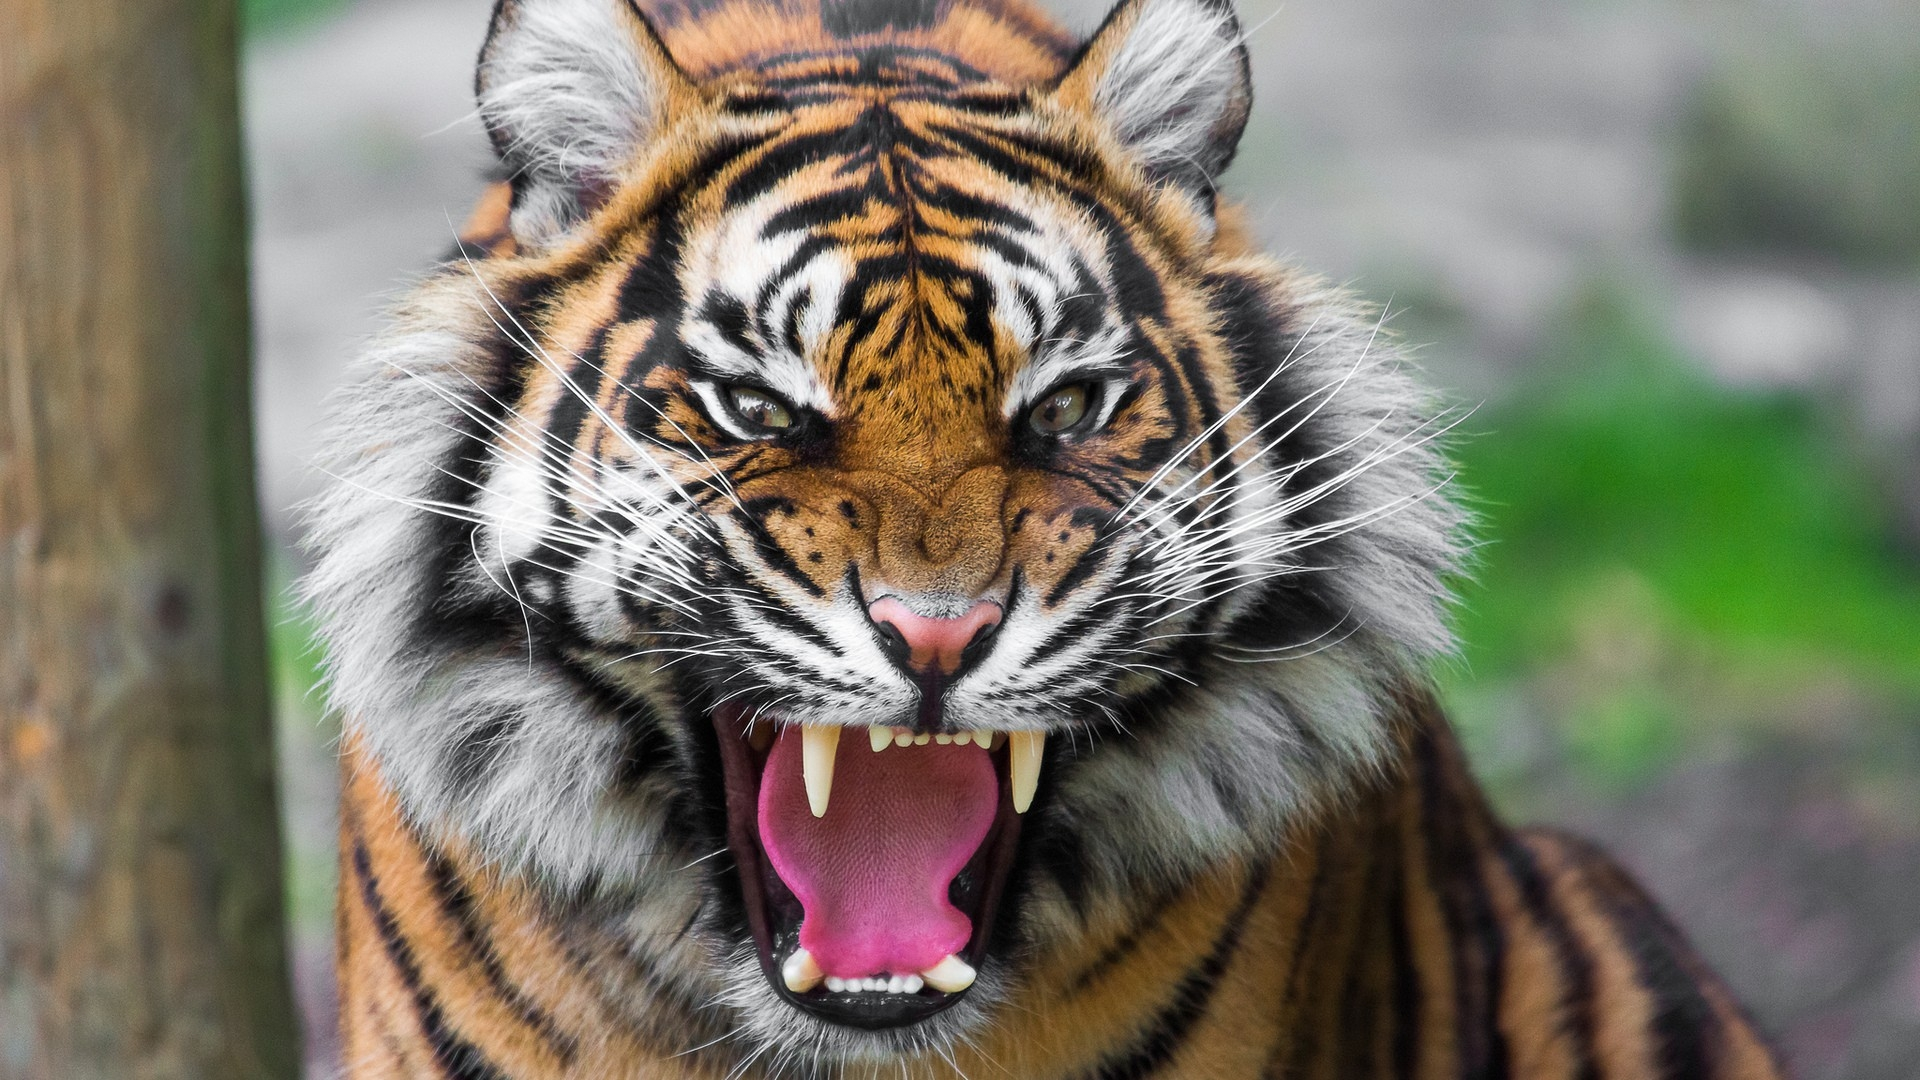
\includegraphics[scale=0.2]{tiger.jpg}
\caption{Tygrys bengalski}
\end{figure}

\subsection{Tabela}
\begin{table}[h!]
\caption{województwa}
\centering
\label{tab:wojewodztwa}
\begin{tabular}{|c|c|c|}
	\hline 
	\textbf{województwo} & \textbf{ludność}(2016) & \textbf{powierzchnia}[$ km^2 $]\\
	\hline
	wielkpolskie & 3 475 323 & 29 826,50 \\
	\hline
	zachodniopomorskie & 1 710 482 & 22 892,48 \\
	\hline
	lubuskie & 1 018 084 & 13 987,93 \\
	\hline
	łudzkie & 2 493 603 & 18 218,95 \\
	\hline
\end{tabular}
\end{table}
\newpage

\section{Zadanie 7}
\begin{enumerate}[label=(\alph*)]
	\item {\LARGE $ {n\choose k} = \frac{n!}{k!(n-k)!} $}
	\item {\Large $ a^2 + b^2 = c^2 $}
	\item {\LARGE $ \frac{\frac{1}{2}+\frac{1}{4}}{\frac{1}{8}}\neq1 $}
	\item {\LARGE $ \sum_{i=1}^{n}i^2 = \frac{n(n+1)2n+1}{6} $}
	\item {\LARGE $ C_2^{-3} + O_2^0 \rightarrow C^{+4}O_2^{-2} + H_2^{+1}O^{-2} $} 
	\item $ A_{m,n}   = $
	
	$\begin{bmatrix}
		a_{1,1} & a_{1,2} & \dots & a_{1,n} \\
		a_{2,1} & a_{2,2} & a_{2,3} & \dots  & a_{2,n} \\
		\vdots & \vdots & \vdots & \ddots & \vdots \\
		a_{m,1} & a_{m,2} & a_{m,3} & \dots  & a_{m,n}
	\end{bmatrix}$
	
	
\end{enumerate}
\newpage

\section{Zadanie 8}
\noindent
\enquote{Ciemno wszędzie, głucho wszędzie,\\ Co to będzie, co to będzie?}\cite{mickiewicz1992dziady}\\\\
\enquote{było to bardzo piękne zwierzę ,które miało złote poroże i racice ze spiżu}\cite{parandowski1989mitologia}\\

\bibliographystyle{plain}
\bibliography{references}

\end{document}